\documentclass[11pt, oneside]{article} 
\usepackage{geometry}
\geometry{letterpaper} 
\usepackage{graphicx}
	
\usepackage{amssymb}
\usepackage{amsmath}
\usepackage{parskip}
\usepackage{color}
\usepackage{hyperref}

\graphicspath{{/Users/telliott/Github-math/figures/}}
% \begin{center} \includegraphics [scale=0.4] {gauss3.png} \end{center}

\title{Proof Without Words:  trigonometry}
\date{}

\begin{document}
\maketitle
\Large

%[my-super-duper-separator]

Here is a proof without words for $\tan 22.5^\circ = \sqrt{2} - 1$:
\begin{center} 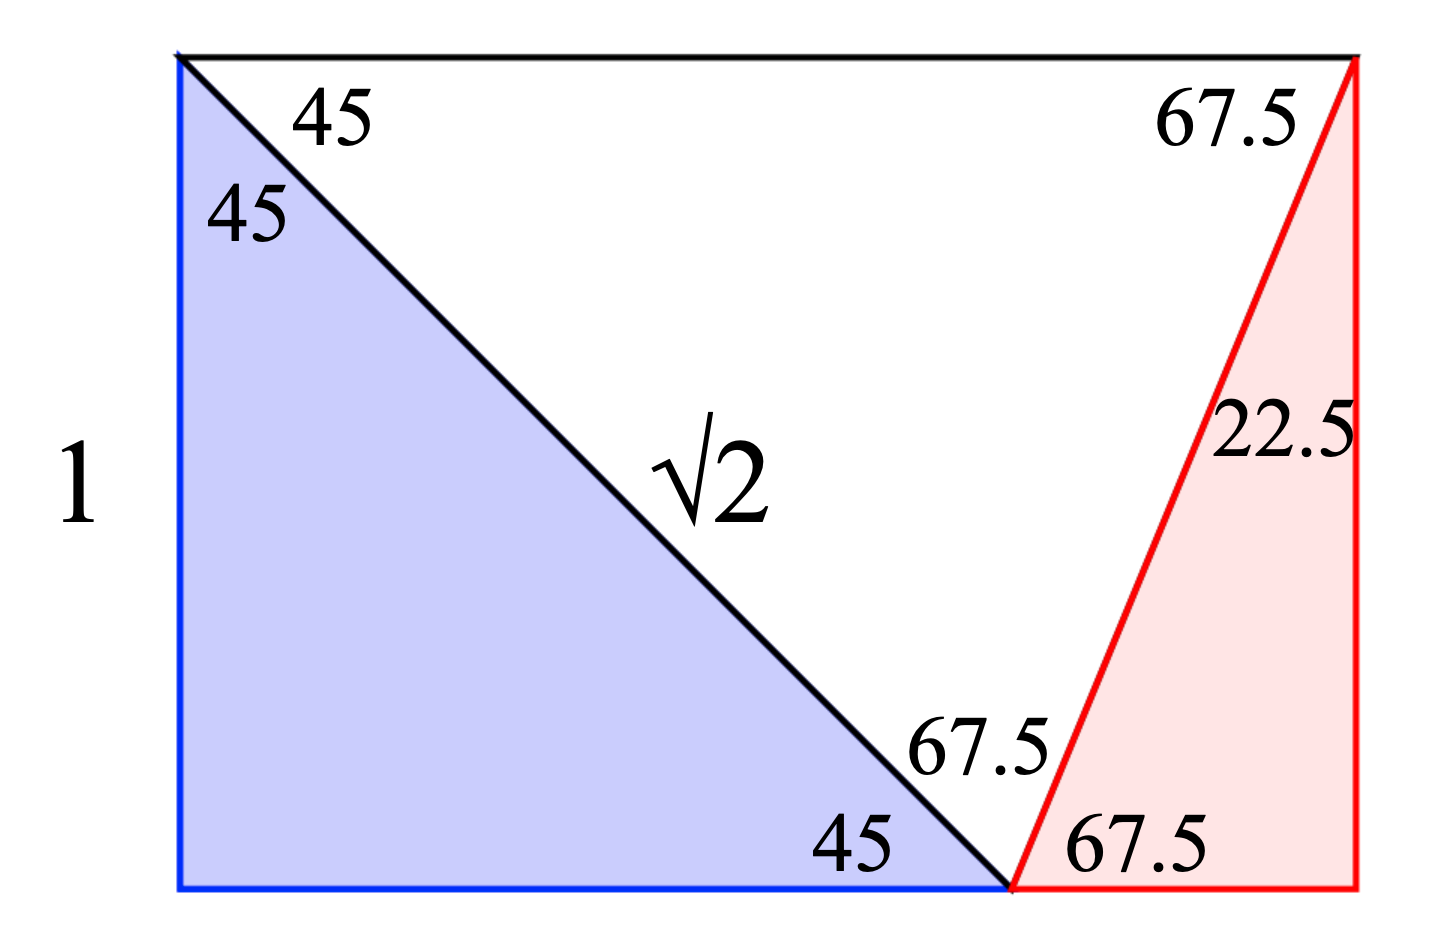
\includegraphics [scale=0.3] {pwow1_label.png} \end{center}

And a derivation.  The standard double-angle formulas:
\[ \sin 2A = 2 \sin A \cos A \]
\[ \cos 2A = \cos^2 A - \sin^2 A \]

When $A = 22.5^\circ$, the left-hand sides are equal so
\[ 2 \sin A \cos A = \cos^2 A - \sin^2 A \]
\[ 2 \tan A = 1 - \tan^2 A \]

Let $t = \tan A$
\[ 2t = 1 - t^2 \]
\[ t^2 + 2t - 1 = 0 \]
\[ t = \frac{-2 \pm \ \sqrt{4 + 4}}{2} \]
\[ = -1 \pm \ \sqrt{2} \]
We take the positive root
\[ \tan 22.5^\circ = \sqrt{2} - 1 \]

And here is another proof without words for the general case:

\begin{center} \includegraphics [scale=0.4] {pwow4_label.png} \end{center}
\[ \tan t = \frac{\sin 2t}{1 + \cos 2t} = \frac{1 - \cos 2t}{\sin 2t} \]

When $2t = 45^\circ$, then the sine and cosine are both $1/\sqrt{2}$.  Multiply on top and bottom to obtain $\tan t = \sqrt{2} - 1$.


\end{document}